\documentclass{thesis-ekf}
\usepackage[T1]{fontenc}
\PassOptionsToPackage{defaults=hu-min}{magyar.ldf}
\usepackage[magyar]{babel}
\usepackage{amssymb,amsthm,pdfpages,listingsutf8}
\footnotestyle{rule=fourth}
\usepackage[dvipsnames]{xcolor}
%\newtheorem{tetel}{Tétel}[chapter]
\theoremstyle{definition}
%\newtheorem{definicio}[tetel]{Definíció}
\theoremstyle{remark}
\newtheorem{megjegyzes}{Megjegyzés}


\lstdefinestyle{json}{
	backgroundcolor=\color{gray!20},
	stringstyle=\color{red},
	keywordstyle=\color{blue},
	keywordstyle=\color{purple},
	numbers=left,
	numberstyle=\tiny\color{gray},
	stepnumber=1,
	numbersep=5pt,
	showspaces=false,
	showstringspaces=false,
	showtabs=false,
	frame=single,
	rulecolor=\color{black},
	tabsize=2,
	breaklines=true,
	breakatwhitespace=true,
	captionpos=b
}

\begin{document}
	
	\institute{Matematikai és Informatikai Intézet}
	\title{Moduláris Plug \& Play IoT / okos~otthon rendszer}
	\author{Farkas Levente\\Program tervező informatikus BSc}
	\supervisor{Dr. Geda Gábor\\egyetemi docens}
	\city{Eger}
	\date{2025}
	\maketitle
	\tableofcontents
	\chapter*{Bevezetés}
	\addcontentsline{toc}{chapter}{Bevezetés}
	
	Az emberi faj a létezésétől kezdve lusta volt és lesz. Minden nap valamivel könnyebbé, egyszerűbbé akarjuk tenni a mindennapokat, hogy minél kevesebbel keljen foglalkoznunk és több időt tölthessünk más tevékenységgel. Az okos otthon rendszerek pontosan ezt teszik lehetővé, ezek régen drágák voltak így csak a tehetősebb emberek engedhették meg maguknak. Ma azonban olcsóbb ökoszisztémák is léteznek, de még így sem tudják sokan megfizetni. A projekt amiről ezen dolgozat szól egy olcsóbb, közösség alapú ökoszisztéma létrehozását tűzte ki célul.
	
	Számomra elképesztő belegondolni abba, hogy pár sor kóddal ki tudunk hatni a környezetünkre. Főképp azért, mert a programozás szempontjából én mindig adatkezelésként tekintettem a munkánkra. Még a szakdolgozat témájának kiválasztása előtt kapcsolatba kerültem a mikrokontrollerek világával és attól a ponttól nem tudtam elengedni ezen eszközök varázsát. Tekintettel arra, hogy az áramkörök és elektromosság foglalkoztatott hobbi szinten már régóta, ez egy nagyszerű lehetőség volt, hogy kettő nagy szenvedélyemet, az informatikát és az áramköröket ötvözzem a szakdolgozatomban. Számomra hihetetlen volt akár csak egy LED\footnote{Light Emitting Diode, avagy fényt kibocsájtó dióda.} villanása is.
	
	Szakdolgozatom termék-orientált. Célja az, hogy a kevésbé tehetős emberek számára is elérhetővé tegye az okos otthonok varázsát. Logikám szerint az okos eszközök árát nagyrészt a programozható mikrochipek teszik ki, ezeknek egy részről a hozzá tartozó áramkört kell vezérelniük, amely nem egy nehéz feladat, azonban az adatnak amely alapján ez működni fog valahogy el kell jutnia az eszközhöz, ez WiFi-n keresztül történik minden esetben, azonban így jelentősen megugrik ezek ára. A gondolatmenetemben egy egy eszközt képzeltem el, amely ezt a drága technológiát központosítja, ezzel a rendszer szummázott árát csökkentve.
	
	Az eszköz önmagában nem képes sok mindenre, azonban a hozzá kapcsolódó ,,buta'' modulok használatával lehetőség nyílik arra, hogy egy eszköz négy modult, azaz működésében különálló okos eszközt kezeljen.
	A fejlesztés idejében az eszköz négy modult képes befogadni, azonban ez áramkör és program módosítással növelhető.
	
	Számomra fontos volt még az általam nem ismert, vagy nem használt technológiák használata, így próbáltam minél több számomra új technológiát használni, ezekről a technológiákról bővebben a \ref{ch_tech}.~fejezetben olvashatnak.
	\chapter{Technológiák}
	\label{ch_tech}
	\section{Eszköz oldal}
	\subsection{Programozási nyelv}
	Ahogy később a \aref{ch_esp}.~fejezet \aref{se_espB}.~szekciójában olvashatja az ESP32 eszközöket C/C++ nyelveken lehet főképp programozni, ezek mellett script nyelveket is lehet használni.
	
	A megoldásban első sorban C++ nyelvet akartam használni, azonban ez a megközelítés felvetett számos problémát a megvalósítás közben (ezekről bővebben a \aref{sub_fejlESP}.~alszekcióban olvashat). A problémák hatására elhagytam a C++ programozási nyelvet és MicroPython-ra váltottam.
	
	A ESP32\_GENERIC\_S3-SPIRAM\_OCT-20241129-v1.24.1 firmware-en történt a fejlesztés a váltás eredményeként. Ez elérhető a \href{https://micropython.org/download/}{MicroPython} weboldalán.
	\subsection{IDE}
	Alapvetően a Visual Studio Code volt a választott IDE a fejlesztéshez, azonban ez bármely extensiont próbáltam használni egyik sem tudta sikeresen feltölteni a programot az ESP-re. Így a fejlesztés első szakaszában a VSCode-ban megírt programot az Arduino IDE segítségével töltöttem fel.
	
	A programozási nyelv váltása után a VSCode továbbra sem volt működőképes. Miután a probléma megoldására általam ismert módszerek tárháza kifogyott elkezdtem egy másik IDE után keresni. A keresésem eredményeként rátaláltam egy weblapra\footnote{\url{https://randomnerdtutorials.com/micropython-ides-esp32-esp8266/}} ahol több fejlesztői környezetet említenek. A keresés folyamatában számos GitHub és StackOverflow beszélgetést néztem át válasz után kutatva. Ezekben a beszélgetésekben többször is említették a \href{https://thonny.org/}{ThonyIDE}-t. Ennek eredményéül kezdtem el használni az említett környezetet.
	\section{API}
	Szerencsére az API-hoz használt technológiával nem volt probléma, így ez Node.js-ben íródott Visual Studio Code felhasználásával. Ezt már használtam így nem tartalmazott különösebb meglepetést a fejlesztés.
	\section{Adatbázis}
	A MongoDB egy nyílt forráskódú, dokumentumorientált NoSQL adatbázis, amelyet skálázható és nagy teljesítményű alkalmazások fejlesztésére terveztek. A hagyományos relációs adatbázisokkal (pl. MySQL, PostgreSQL) ellentétben a MongoDB nem táblákban, hanem rugalmas, JSON-szerű dokumentumokban tárolja az adatokat. Ez lehetővé teszi a gyors és hatékony adatkezelést, különösen olyan esetekben, amikor az adatok szerkezete dinamikus vagy változó.
	
	Fő jellemzői a MongoDB-nek:
	\begin{enumerate}
		\item Dokumentumorientált adatmodell:
		\begin{itemize}
			\item Az adatokat BSON (Binary JSON) formátumban tárolja, ami egy bináris reprezentációja a JSON-nek.
			\item Egy dokumentum egy kulcs-érték párokból álló struktúra, amely hasonlít a programozási nyelvekben használt objektumokhoz.
			\item Példa egy dokumentumra:\lstinputlisting[style=json,label=lst_docu,caption={Egy teszt dokumentum az adatbázisból.}]{docu.json}
		\end{itemize}
		\item Rugalmas séma:
		\begin{itemize}
			\item A MongoDB nem követeli meg, hogy minden dokumentumnak ugyanaz a szerkezete legyen. Ez lehetővé teszi, hogy különböző típusú adatokat tároljunk ugyanabban a gyűjteményben (collection).
			\item Például egy users gyűjteményben lehetnek olyan dokumentumok, amelyeknek nincs age mezője, vagy más mezők is lehetnek.
		\end{itemize}
		\item Skálázhatóság:
		\begin{itemize}
			\item A MongoDB horizontálisan skálázható, ami azt jelenti, hogy az adatbázis több szerverre (shard) osztható szét, hogy kezelni tudja a nagy mennyiségű adatot és a magas terhelést.
			\item Támogatja a replikációt is, ami magas rendelkezésre állást és hibaelállást biztosít.
		\end{itemize}
		\item Teljesítmény:
		\begin{itemize}
			\item A MongoDB gyors adatelérést biztosít indexek használatával. Többféle indexet támogat, beleértve az egyszerű, összetett, szöveges és geospatial indexeket.
			\item A memóriában történő adatkezelés (in-memory storage) tovább növeli a teljesítményt.
		\end{itemize}
		\item Aggregáció és lekérdezés:
		\begin{itemize}
			\item A MongoDB hatékony lekérdezési nyelvet (Query Language) és aggregációs keretrendszert (Aggregation Framework) biztosít az adatok elemzéséhez és feldolgozásához.
		\end{itemize}
	\end{enumerate}
	A MongoDB továbbá támogatja a CRUD műveleteket (Create, Read, Update, Delete), valamint a tranzakciókat is (a 4.0 verziótól kezdve).\cite{bib_mongo_sql}
	Míg nem kényszeríti a MongoDb sémák használatát van rá lehetőségünk. A sémákban megadhatunk kötelező mezőket, azok típusát, valamint ezekhez köthetünk különböző ellenőrzéseket.
	\lstinputlisting[style=json,label=lst_schema,caption={Felhasználó collection sémája az adatbázisból. (A séma mezőinek azonosítója nem felelnek meg a json nyelv szabájainak, mivel a fájl tartalma konzolban került bevitelre.)}]{user_schema.json}
	
	Ahogy a \ref{lst_schema}.-es példában is látható típus és mező megszorításokat eszközöltem, e mellett az email mező még reguláris kifejezéssel is vizsgálva van.
	\subsection{MongoDB struktúrája}
	A MongoDB az adatbázison belül táblák helyett collection-ök vannak, ezen belül rekordok, avagy sorokkal ellentétben dokumentumokat találunk, ahol oszlopok helyett mezők vannak, az összehasonlítást egy hagyományos SQL adatbázissal a \ref{img_sql_mongo}.~ábrán lehet látni. \cite{bib_mongo_sql}
	 \begin{figure}[!h]
	 	\centering
	 	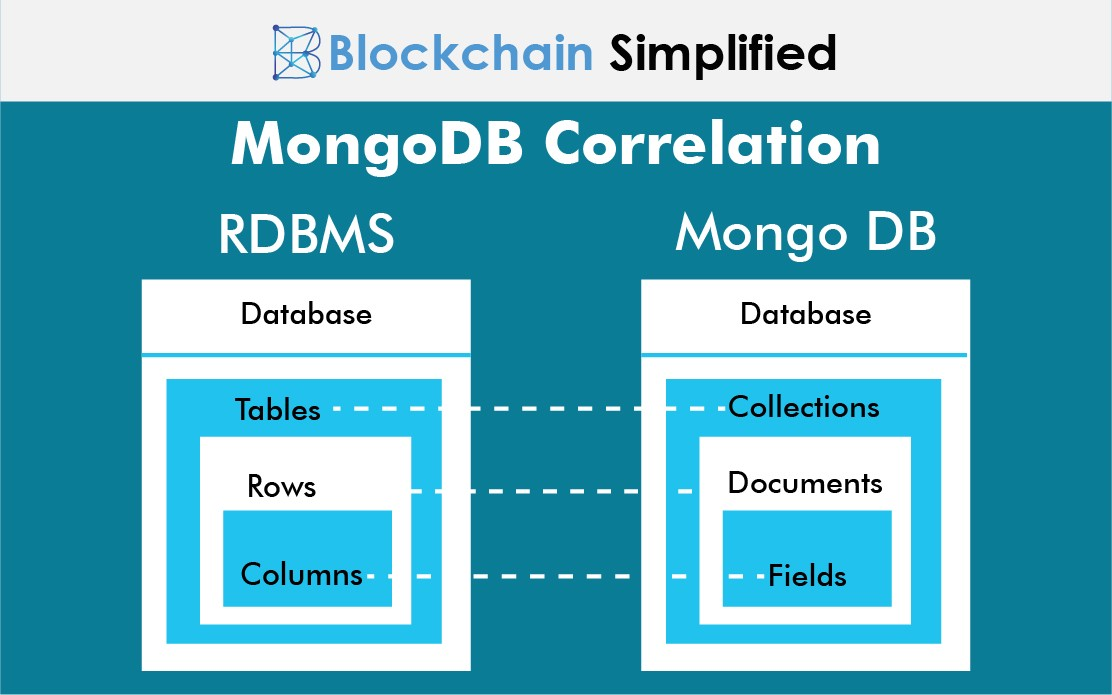
\includegraphics[width=8cm]{mongo_vs_sql}
	 	\caption{SQL adatbázis és MongoDB szerkezeti hasonlóságai.}
	 	\label{img_sql_mongo}
	 \end{figure}
	\section{Frontend technológia}
	Az eszköz hatékony vezéréléséhez szükségünk van egy applikációhoz, azonban lehet, hogy egyes emberek nem mindenhez a telefonjukat akarják használni. Ez problémát vet fel, mivel több kódbázis fenntartása és javítása sok embert és erőforrást igényel. 
	
	\textbf{Megoldás:} Olyan keretrendszerre, vagy programozási nyelvre van szükség, amely működőképes több platformon is.
	
	\textbf{Például:}
	\begin{itemize}
		\item React Native
		\item Kotlin
		\item Flutter
		\item Lynx
	\end{itemize}
	\begin{megjegyzes}
		A legújabb keretrendszer a LynxJs, amely 2025.03.05.-én jelent meg. Ahogy a React Native ez is javascript alapú, így a Lynx és React Native egyfajta versenyhelyzetben vannak. A keretrendzerek összehasonlítását olvashatja a  \href{https://medium.com/@mostsignificant/introducing-lynx-how-tiktoks-new-framework-compares-to-react-native-580a52d3462c}{Medium.com}-on, valamint a \href{https://lynxjs.org/}{LynxJs.org}-on tudhat meg többet a keretrendszerről.
	\end{megjegyzes}
	Választásom a Flutter-re esett. 
	\subsection{Miért Flutter?}
	\begin{itemize}
		\item könnyű crossplatform build lehetőség
		\item opensource
		\item gyorsaság\footnote{,,Flutter is powered by Dart, a language optimized for fast apps on any platform''\cite{bib_flutter_web}}
		\item új technológia megismerése
	\end{itemize}
	\subsection{Flutter ismertetése}
	A Flutter egy olyan eszköz, amely lehetővé teszi a fejlesztők számára, hogy natív, többplatformos alkalmazásokat hozzanak létre egyetlen programozási nyelv és egyetlen kódbázis segítségével. Nem olyan alkalmazást hoz létre, amely böngészőben fut, vagy amelyet natív alkalmazásokba csomagolnak. Ehelyett natív alkalmazásokat készít iOS-re és Androidra is, amelyek később közzétehetők az app store-okban.
	
	
	Az alkalmazást létrehozásához egyetlen programozási nyelvre van szükségünk, ahelyett, hogy különböző nyelveket használnánk egy iOS vagy Android alkalmazás fejlesztéséhez. Így csak egyetlen kódbázissal kell foglalkoznunk. A Flutter egy SDK\footnote{Software Development Kit}, amely lehetővé teszi, hogy a kódbázisodat natív gépi kódra fordítsd, amely a fent említett platformokon fut.
	
	
	A fordítási eszközök mellett a Flutter keretrendszerként is funkcionál, UI építőelemeket (widgeteket) biztosít, mint például lapok, legördülő menük, gombok stb., valamint néhány segédfüggvényt és csomagot, amelyeket az SDK segítségével lehet lefordítani.\cite{bib_flutter_short}
	
	Flutter applikációt a fent említettek mellett még Windows-on, Linux-on és Web-en is lehet használni.
	\chapter{ESP32, az eszköz}
	\label{ch_esp}
	\section{ESP32 bemutatása}
	\label{se_espB}
	Az ESP32 egy rendkívül sokoldalú és hatékony mikrokontroller, amely számos területen alkalmazható. Duális magos processzora, integrált Wi-Fi és Bluetooth képességei, valamint gazdag I/O lehetőségei miatt kiváló választás mind IoT, mind ipari vagy okos otthon alkalmazásokhoz. Az ESP32 fejlesztése egyszerű és gyors, köszönhetően a széles körben elérhető fejlesztői eszközöknek és könyvtáraknak. Ezek a tulajdonságok teszik az ESP32-t az egyik legnépszerűbb mikrokontrollerré a beágyazott rendszerek világában.
	
	Az általam \aref{img_myesp} használt modell az ESP32-S3-DevKitC-1 N32R8V, amely egy ESP32-S3-WROOM-2 chipet tartalmaz, ezt az Espressif System fejlesztette ki.
	\begin{figure}[!ht]
		\centering
		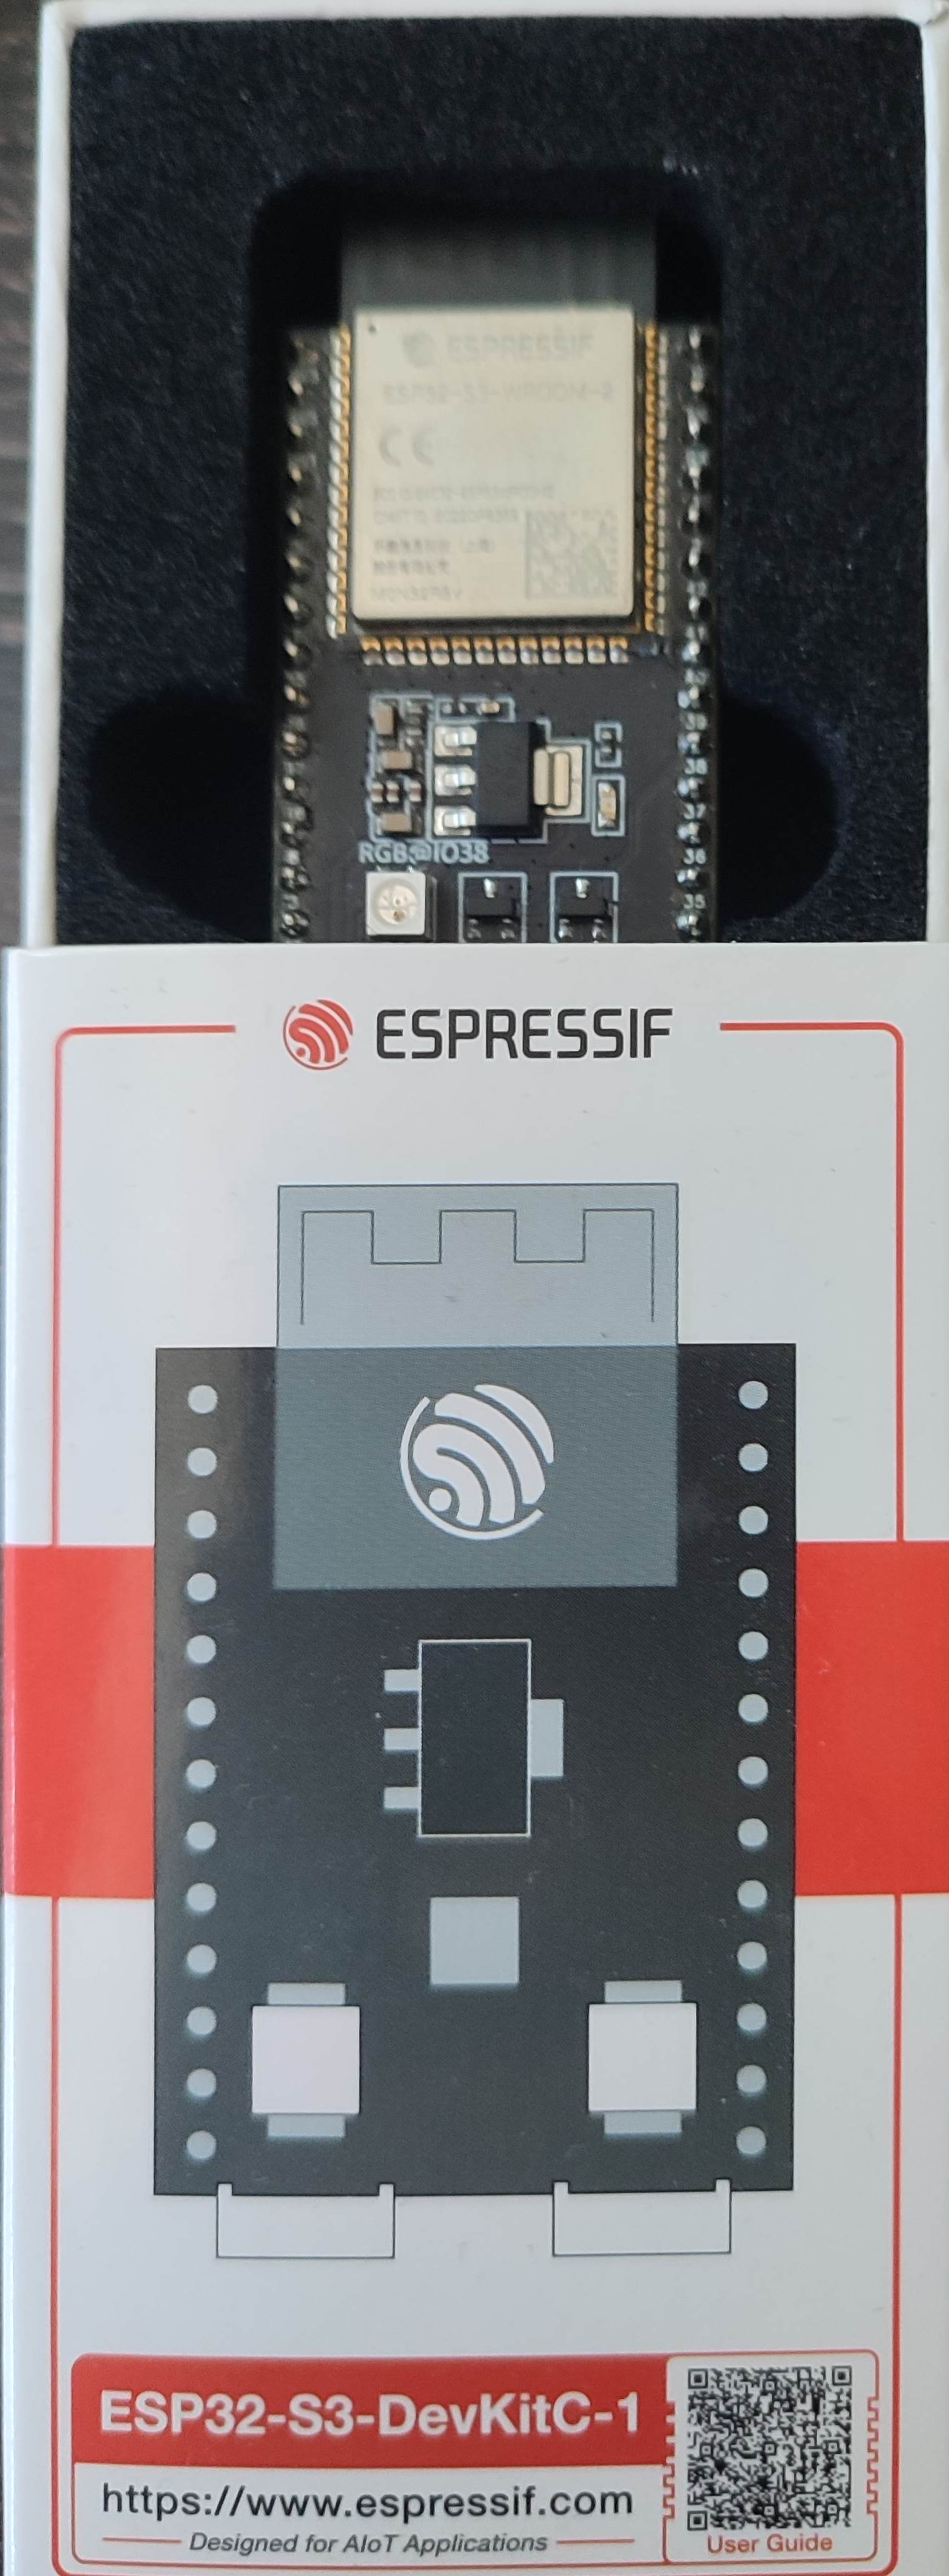
\includegraphics[width=3cm]{MyESP32}
		\caption{Általam használt ESP32 modell}
		\label{img_myesp}
	\end{figure}
	
	Ezen eszközök számos bemeneti és kimeneti perifériákkal rendelkeznek:
	\begin{itemize}
		\item Digitális I/O pin-ek
		\item Analóg bemenetek (ADC\footnote{Analog to Digital Converter, lehetővé teszi az áramkörben érzékelt analóg jelek feldolgozását.})
		\item Digitális-analóg átalakítók (DAC\footnote{Digital to Analog Converter, lehetővé teszi az áramkörre kibocsájtott feszültség modulálását.})
		\item PWM (Pulse Width Modulation\footnote{Ezen technológia teszi lehetővé a DAC működését.}) kimenetek
		\item SPI, I2C, UART kommunikációs interfészek
	\end{itemize}
	Ezek a csatlakozók lehetővé teszik különböző érzékelők, kijelzők és egyéb perifériák csatlakoztatását.
	Ezeket az eszközöket nagyrészt C és C++ nyelven lehet programozni, azonban van lehetőség a MicroPython és Lua script nyelvek használatára.
	\section{Fejlesztés}
	\subsection{Hardver szintű fejlesztés}
	A projekt megvalósításához szükség volt egy egyedi áramkörre, amivel maximalizálhatom az elérhető portok számát.
	\begin{figure}[!ht]
		\centering
		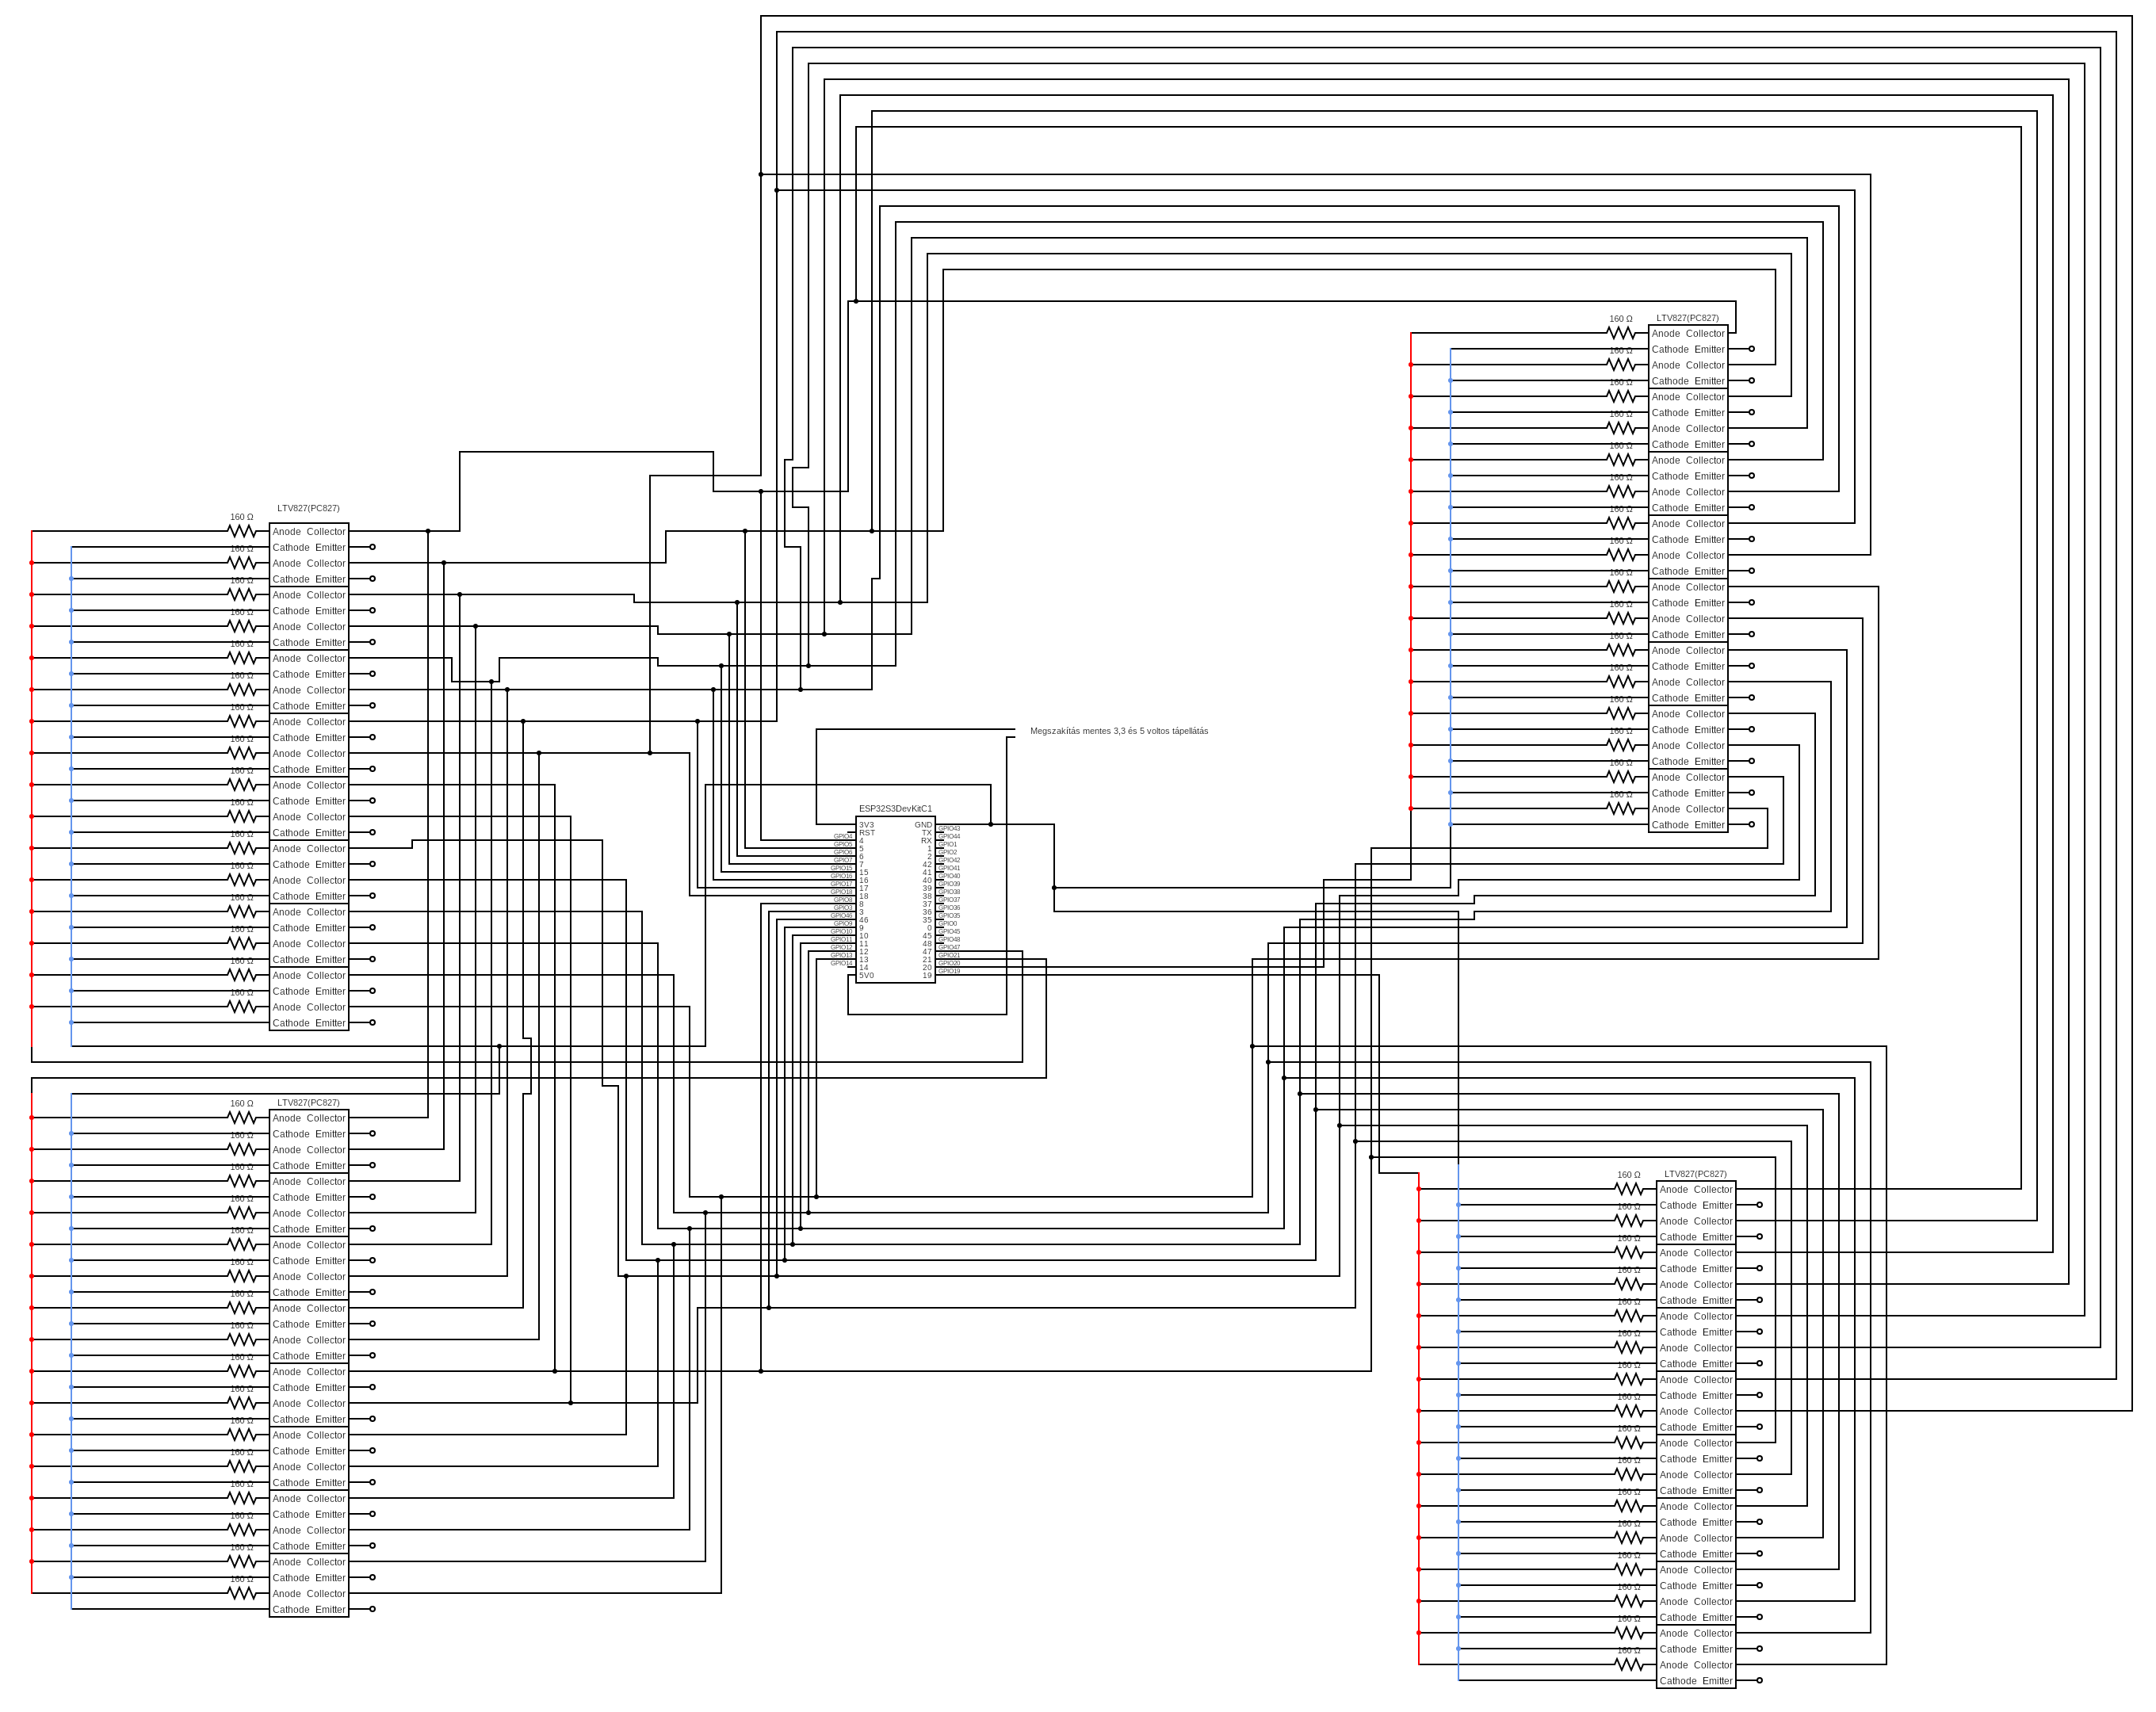
\includegraphics[width=10cm]{circuit}
		\caption{Egyedi áramkör}
		\label{img_circ}
	\end{figure}
	A \ref{img_circ}-es ábrán látható az említett áramkör, amely segítségével elérem az általam elfogadható eredményt. Ebben a fő alkatrész az optocsatoló, amellyel igyekeztem  az esetleges interferenciát csökkenteni.
	
	Ez a diagram a \href{https://www.circuit-diagram.org/}{Circuit Diagram} segítségével készült.
	Az ábra nem tartalmazza az érzékelő vezetékeket, amivel az eszköz érzékeli, hogy csatlakoztatva van-e a modul.
	\subsection{Szoftver fejlesztése és feltárt problémák}
	\label{sub_fejlESP}
	Fejlesztés elején több probléma is felmerült.
	\begin{enumerate}
		\item A modul vezérlő fájlok tárolása. Amennyiben C++ vagy C nyelvet használunk a belső tárhely kizárólagosan az általunk feltöltött fájlokat tartalmazza és a hozzáférés nehézkes fájlrendszer nélkül. Szerencsére elérhető több csomag is ennek a megoldására, mint a \href{https://github.com/littlefs-project/littlefs}{LittleFS}, vagy a \href{https://docs.espressif.com/projects/esp-idf/en/stable/esp32/api-reference/storage/spiffs.html}{Spiffs}
		\item A modul vezérlő fájlok használata, vagy futtatása. A projekt egyik fő feladata, hogy a modulok programja és a fő program egymástól függetlenül legyenek képesek működni, azaz ne a fő program hajtsa végre a szükséges lépéseket, hanem a modul vezérlő. Egy megoldás erre a fájl dinamikus betöltése és a program belépési pontjának meghatározása, majd a pont memória címén keresztüli futtatás. Ez a megközelítés a programot rendkívül bonyolultá tette volna és memória biztonsági problémákat is felvetett volna, mivel a C++ nyelvben íródó programnak C-t is használnia kellett volna.
	\end{enumerate}
	 Ez a kettő komolyabb probléma vezetett arra, hogy más nyelvet keressek. A MicroPython mind a kettő problémára megoldást nyújtott a beépített fájlrendszerével és JIT\footnote{Just In Time} interpreterével, ugyanis így nem bináris kóddal kell dolgozni, hanem egyszerű \textit{.py} fájlokkal.
	 Ez a változtatás nagyban megkönnyítette a program fejlesztését.
	 
	 A váltás után neki tudtam kezdeni a tényleges fejlesztésnek. Itt a főbb problémákat a fájl letöltése és azoknak a futtatása jelentette. A fájl letöltését több módszerrel is megkíséreltem, a Google API használatával sikeresen le tudtam tölteni a fájlt az API mindössze az igényelt API kulcsot és a fájl azonosítóját kéri (Az azonosító a megosztási linkből kinyerhető.).
	 
	 Ezen a ponton a szerverrel való kommunikáció is kérdéses volt. Elsőre Websocket technológiát terveztem használni, azonban ezt drágának találtam és a szervernek egyszerre több kapcsolatot is fenn kellett volna tartania, miközben relatívan kevés és ritka az információ áramlása. A következő ötlet egy az eszközön futó API volt, ez azonban ennek a megoldásnak, hogy működőképes legyen szükséges az eszköz IP címe, valamint esetlegesen portforwarding-re van szükség amely nem egyezik az eszköz Plug\&Play irányzatával. Ennek eredményéül a jól ismert RestAPI technológia mellett döntöttem. Az API-ról többet olvashat a \ref{ch_API}. fejezetben.
	 
	 API-ra még így szükség van a konfigurációhoz, ehhez a Microdot könyvtárat használtam, valamint a szerver felé irányuló kérésekhez a urequests és az abból származó adatok feldolgozásához a nyelv által alapértelmezetten tartalmazott modulokat használtam. A beépített NeoPixel LED használatához a NeoPixel könyvtárra volt szükségem.
	 \subsection{Működése}
	 Az eszköz használata konfigurációval kezdődik, melyet kék fénnyel jelez a felhasználónak. A konfiguráció után megpróbál csatlakozni a megadott hálózathoz eközben az eszközön található LED kék fényről pulzáló zöld fényre vált. Amennyiben a kapcsolódás sikeres az eszköz zöld fénnyel jelzi ezt, ha sikertelen, akkor újraindul a folyamat.
	 
	 Sikeres kapcsolódás után önmagát regisztrálja az eszköz a hálózatra. Innentől az eszköz használatra kész és azonnal kérést küld az API-nak a hozzá kapcsolt feladatok iránt érdeklődve. A szerver válasza alapján a következő műveleteket végezheti el az eszköz:
	 \begin{itemize}
	 	\item ,,add\_new'': A parancs kiadásával új modult tudunk hozzáadni az eszközhöz.
	 	\item ,,remove'': Az ,,add\_new'' parancs ellentettje. Modul eltávolítására adja ki a parancsot.
	 	\item ,,disown'': Gyári visszaállítás.
	 	\item ,,network\_reset'': Az eszköz elfelejti a hálózatot. Hasznos lehet, ha az eszközt egy másik épületbe helyezzük át.
	 	\item ,,module\_reset'': Az eszköz belső állapotát visszaállítja, ezzel egyszerre az összes modul eltávolítható.
	 	\item ,,run'': Futtatja a modulhoz megadott programot.
	 \end{itemize}
	 Fontos megjegyezni, hogy minden feladat elvégzése annak törlésével és egy új kéréssel záródik. A ,,run'' parancs esetén az eszköz a modul azonosítója alapján dönti el, hogy melyik modult kell használnia, azaz megállapítja a modul áramkörét és kiválasztja azt. Az ,,add\_new'' esetén az eszköz újraindul, hogy a program sikeresen érzékelni tudja a fájl változásait, erre a ,,remove'' parancs esetén nincs szükség, mivel a program belső állapota változik csak.
	 
	  Az eszköz esetleges áramkimaradásra fel van készítve, mivel a belső állapot változása folyamatosan mentve van a belső tárhelybe.
	\chapter{API}
	\label{ch_API}
	
	\chapter{Frontend}
\begin{thebibliography}{8}
	\bibitem{bib_mongo_sql}A szekció a \href{https://blockchainsimplified.com/blog/mongodb-introduction/}{Blockchain Simplified} és a DeepSeek alapján és felhasználásával készült.
	[Letöltve/látogatva:2025.03.21]
	\bibitem{bib_flutter_web}\url{https://flutter.dev/}
	[Letöltve/látogatva:2025.03.23]
	\bibitem{bib_flutter_short}\url{https://www.fullstack.com/labs/resources/blog/an-introduction-to-flutters-world} fordítva DeepSeek által.
	[Letöltve/látogatva:2025.03.23]
\end{thebibliography}
\end{document}